% !TEX root = ../main.tex

%----------------------------------------------------------------------
\subsection{In-distribution performance (Tier~0)}\label{sec:id}
%----------------------------------------------------------------------

Table~\ref{tab:main} summarizes \dart{}'s performance against baselines on
the IMP2D test set (1\,065 samples).

\begin{table}[t]
\centering
\caption{Test-set performance on IMP2D (Tier~0, random split).
  $\Delta_\mathrm{ALIGNN}$ is relative MAE reduction vs.\ ALIGNN.
  CrystalTransformer$^*$ uses the same backbone as \dart{} but without
  the defect-site embedding or optimized training recipe.}
\label{tab:main}
\begin{tabular}{@{}lrcc@{}}
\toprule
Model & Params & MAE (eV) & $\Delta_\mathrm{ALIGNN}$ \\
\midrule
Naive (global mean)  & ---     & 2.302 & --- \\
LightGBM (ours)      & ---     & 1.158 & --- \\
El~Alouani~\textit{et al.} & --- & 0.518 & $+4\%$ \\
SchNet               & 0.46\,M & 0.585 & $+8\%$ \\
ALIGNN               & 4.03\,M & 0.540 & --- \\
CrystalTransformer$^*$  & 0.75\,M & 0.516 & $-4\%$ \\
\midrule
\dart{} (single)     & 0.75\,M & \textbf{0.407} & $-25\%$ \\
\dart{} (29-ens.)    & ---     & \textbf{0.359} & $-34\%$ \\
\bottomrule
\end{tabular}
\end{table}

\dart{} achieves a single-model MAE of 0.407\eV{}, reducing the error by
25\% relative to ALIGNN (0.540\eV{}) with 5.4$\times$ fewer parameters
(0.75\,M vs.\ 4.03\,M).
Notably, the vanilla CrystalTransformer backbone---sharing \dart{}'s
architecture but trained with MSE loss and plateau scheduling---reaches
only 0.516\eV{}, confirming that the defect-site embedding and optimized
training pipeline contribute a further 21\% improvement beyond
architectural choice alone.
The 29-model ensemble further reduces the MAE to 0.359\eV{} ($-34\%$),
with multi-source models contributing orthogonal error patterns
(selected at $k=3$ during greedy forward selection).

\paragraph{Computational efficiency.}
\dart{}'s compact design translates to practical training and inference
advantages.
A full 150-epoch training run completes in ${\sim}22$ minutes on a
single NVIDIA L40S GPU, compared to ${\sim}12$ minutes for the
50-epoch CrystalTransformer baseline (at lower final accuracy) and
several hours for ALIGNN with comparable hyperparameter search.
At inference, \dart{} processes the 1\,065-sample test set in
$<5$~seconds, enabling rapid screening of the full
$44\times65$ host--dopant matrix in under 30~seconds.

\paragraph{Error structure.}
Figure~\ref{fig:error_analysis} decomposes prediction errors along three
physically meaningful axes.
(a)~By defect type: adsorbates (0.410\eV{}, $n=724$) and interstitials
(0.401\eV{}, $n=341$) show comparable accuracy, indicating no systematic
bias toward either defect class.
(b)~By $\ef$ magnitude: the model is most accurate for $|\ef| < 5$\eV{}
(MAE $\leq 0.34$\eV{}) but degrades for extreme values
($\ef > 10$\eV{}: MAE $= 2.69$\eV{}, $n=35$).
This degradation reflects three compounding factors: data sparsity in the
tails ($<3.3\%$ of training data), the intrinsic difficulty of high-energy
configurations where DFT convergence itself is often marginal, and the
physical diversity of extreme-$\ef$ structures---which span chemically
disparate host--dopant pairs with qualitatively different bonding
character (ionic vs.\ covalent vs.\ metallic).
(c)~By dopant element: Figure~\ref{fig:periodic_table} maps per-dopant
MAE onto the periodic table, revealing that main-group metals (Bi, Pb,
Sr: MAE $< 0.17$\eV{}) are consistently easier to predict than early
transition metals (Sc, Mn, Ta: MAE $> 0.77$\eV{}), suggesting that
partially filled $d$-shells introduce complex multi-orbital hybridization
that challenges the model.

\begin{figure*}[t]
\centering
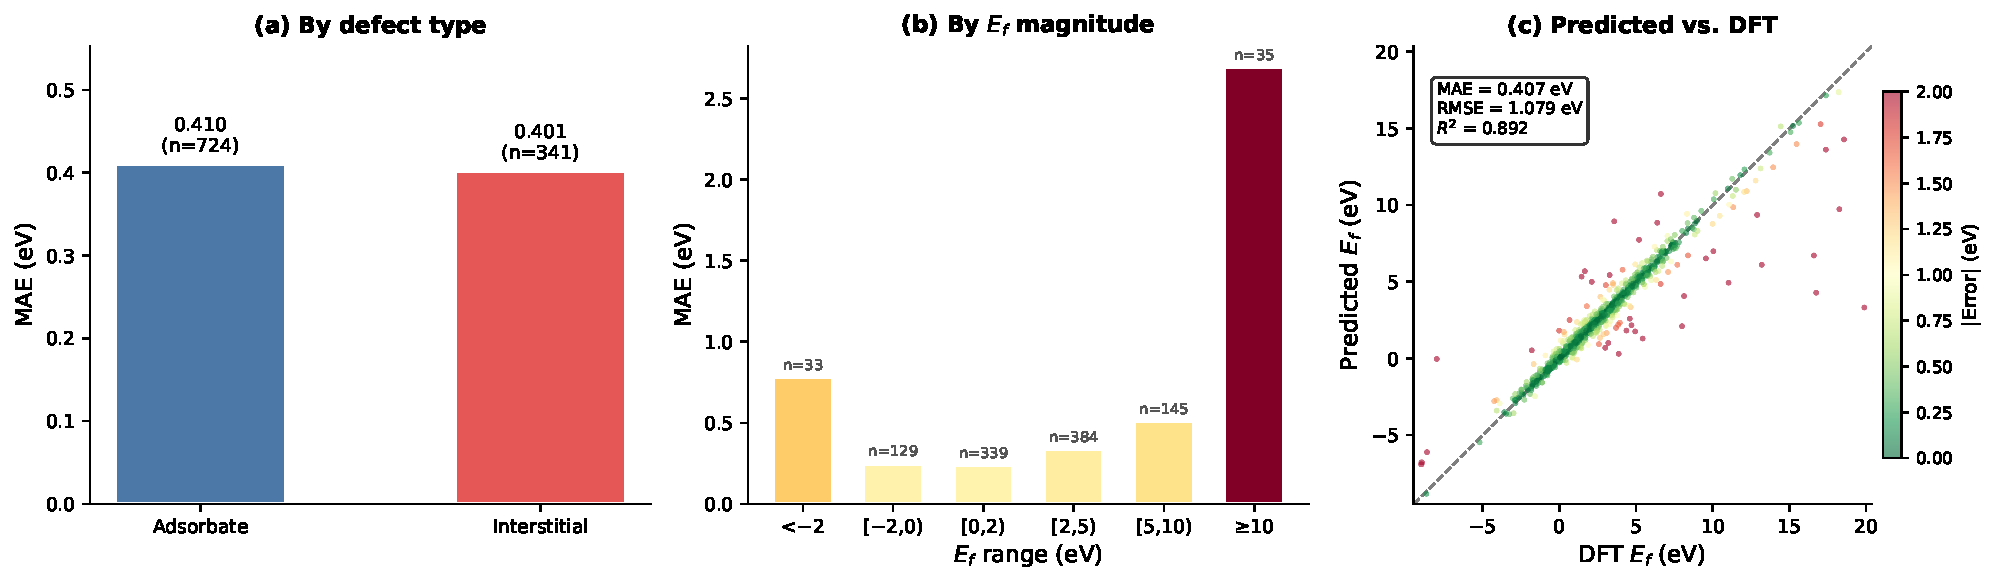
\includegraphics[width=\textwidth]{figures/error_analysis.pdf}
\caption{Error decomposition on the IMP2D test set (1\,065 samples).
  (a)~By defect type: adsorbates and interstitials achieve comparable MAE.
  (b)~By $\ef$ magnitude: performance degrades for $|\ef| > 10$\eV{} due to
  data sparsity.
  (c)~Predicted vs.\ DFT formation energies; color encodes $|\mathrm{error}|$.}
\label{fig:error_analysis}
\end{figure*}

\begin{figure*}[tb]
\centering
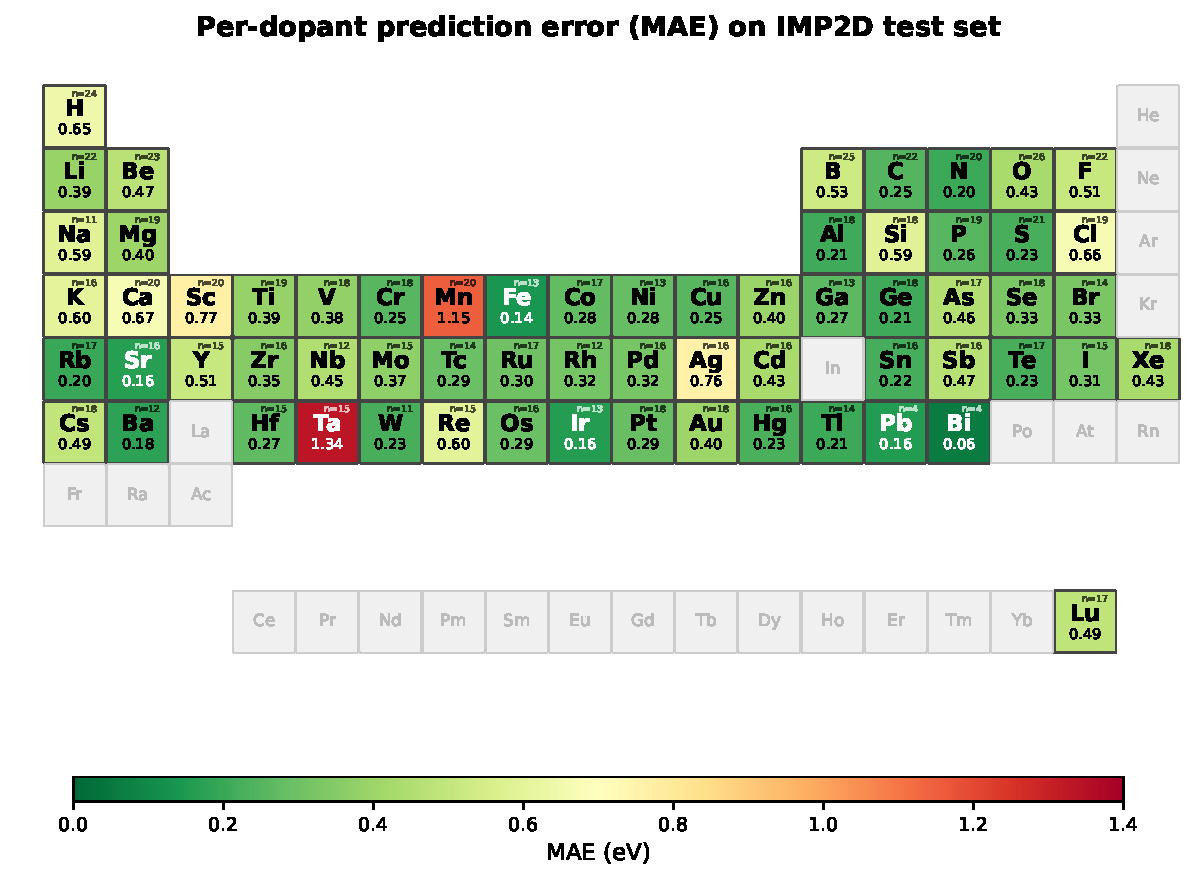
\includegraphics[width=0.92\textwidth]{figures/periodic_table_mae.pdf}
\caption{Per-dopant MAE mapped onto the periodic table.
  Each cell shows the element symbol and MAE (eV); numbers in the top-right
  corner indicate test-sample count.
  Main-group metals (Bi, Pb, Sr) are easiest; early transition metals with
  partially filled $d$-shells (Ta, Mn, Sc) are hardest.
  Grey cells indicate elements absent from the IMP2D test set.}
\label{fig:periodic_table}
\end{figure*}

%----------------------------------------------------------------------
\subsection{Training pipeline ablation}\label{sec:ablation}
%----------------------------------------------------------------------

Table~\ref{tab:ablation} presents a systematic ablation of the training
recipe, with each row adding one component to the previous configuration.
All entries are averages over 3 seeds ($\pm$1 standard deviation).

\begin{table}[t]
\centering
\caption{Cumulative training pipeline ablation (3-seed averages).
  All use the same \dart{} architecture ($d=128$, 3+2 layers).}
\label{tab:ablation}
\begin{tabular}{@{}lccc@{}}
\toprule
Configuration & Seeds & MAE (eV) & $\Delta$ \\
\midrule
MSE loss, plateau LR        & 3 & $0.516 \pm 0.006$ & --- \\
$\to$ MAE (L1) loss          & 3 & $0.474 \pm 0.018$ & $-0.042$ \\
$\to$ + cosine warmup        & 5 & $0.426 \pm 0.011$ & $-0.048$ \\
$\to$ + 150\,ep + SWA        & 3 & $0.415 \pm 0.008$ & $-0.011$ \\
% $\to$ + ct-UAE              & 3 &  TBD              &         \\
\bottomrule
\end{tabular}
\end{table}

The largest single improvement comes from switching MSE to MAE loss
($-0.042$\eV{}), consistent with the heavy-tailed $\ef$ distribution.
Cosine warmup provides a further $-0.048$\eV{}, stabilizing the non-smooth
$\ell_1$ gradient during early training.
Extending training to 150 epochs with SWA adds another $-0.011$\eV{}.
Each improvement is significant across seeds (paired $t$-test, $p < 0.05$
for the first two steps).
Figure~\ref{fig:ablation} visualizes the cumulative improvement.

\begin{figure}[t]
\centering
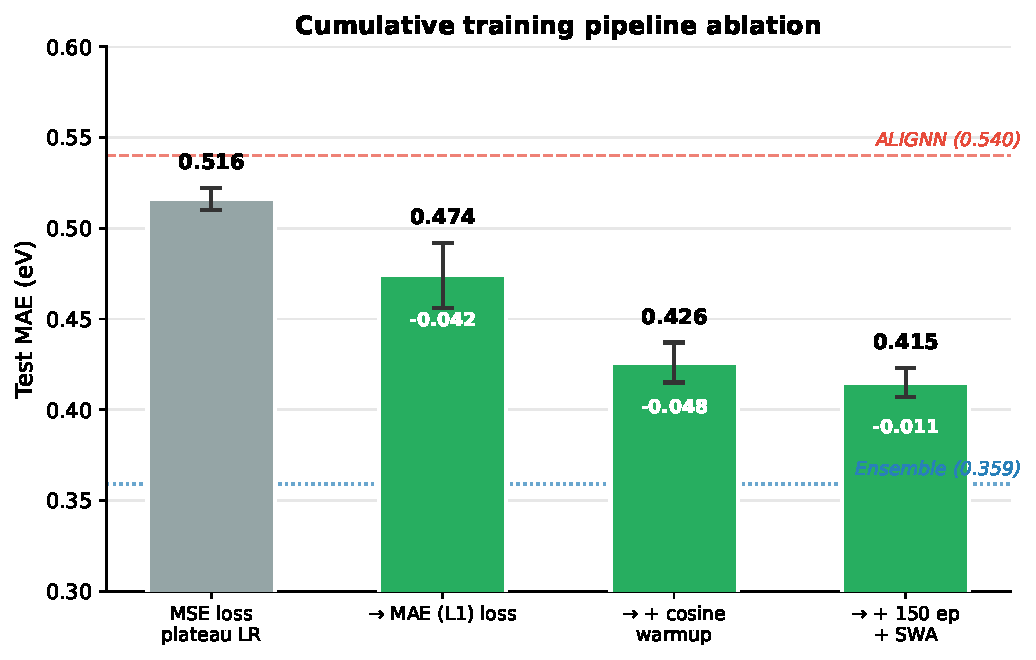
\includegraphics[width=\columnwidth]{figures/ablation_waterfall.pdf}
\caption{Cumulative training pipeline ablation (3--5 seed averages).
  Error bars show $\pm 1\sigma$ across seeds.
  Dashed red line: ALIGNN baseline (0.540\eV{}).
  Dotted blue line: ensemble result (0.359\eV{}).}
\label{fig:ablation}
\end{figure}

%----------------------------------------------------------------------
\subsection{Intra-family OOD evaluation (Tier~1)}\label{sec:ood}
%----------------------------------------------------------------------

Table~\ref{tab:loho} reports the leave-one-host-out (LOHO) results over the
seven G6-TMD hosts.

\begin{table}[t]
\centering
\caption{Tier~1: Leave-one-host-out (LOHO) evaluation on G6-TMDs.
  ``Naive'' is the training-set mean predictor for each fold.}
\label{tab:loho}
\begin{tabular}{@{}lccc@{}}
\toprule
Held-out host & \dart{} MAE & Naive MAE & Ratio \\
\midrule
MoSe$_2$  & 0.377 & 2.874 & 7.6$\times$ \\
MoTe$_2$  & 0.480 & 1.910 & 4.0$\times$ \\
MoSSe     & 0.484 & 2.019 & 4.2$\times$ \\
WTe$_2$   & 0.506 & 2.005 & 4.0$\times$ \\
MoS$_2$   & 0.522 & 3.507 & 6.7$\times$ \\
WSe$_2$   & 0.653 & 2.883 & 4.4$\times$ \\
WS$_2$    & 0.759 & 3.253 & 4.3$\times$ \\
\midrule
\textbf{Mean} & $\mathbf{0.540 \pm 0.117}$ & 2.636 & 4.9$\times$ \\
\bottomrule
\end{tabular}
\end{table}

\paragraph{Graceful degradation.}
Moving from Tier~0 (0.362\eV{}) to Tier~1 (0.540\eV{}) represents a
1.5$\times$ increase in MAE---substantially milder than the naive-baseline
collapse (4.9$\times$ worse than \dart{}).
This indicates that \dart{} has learned transferable representations of
defect--host interactions within the TMD family, not merely memorized
training configurations.

\paragraph{Mo vs.\ W hosts.}
Mo-based hosts (mean MAE $= 0.453$\eV{}) are systematically easier to
predict than W-based hosts (mean MAE $= 0.639$\eV{}).
This asymmetry reflects the greater spatial extent of W $5d$ orbitals
compared to Mo $4d$, leading to more delocalized defect states and
stronger defect--host $d$--$p$ hybridization that is harder to capture from
the remaining training data.
Figure~\ref{fig:loho} compares \dart{} and naive-baseline MAE for each fold.

\begin{figure}[t]
\centering
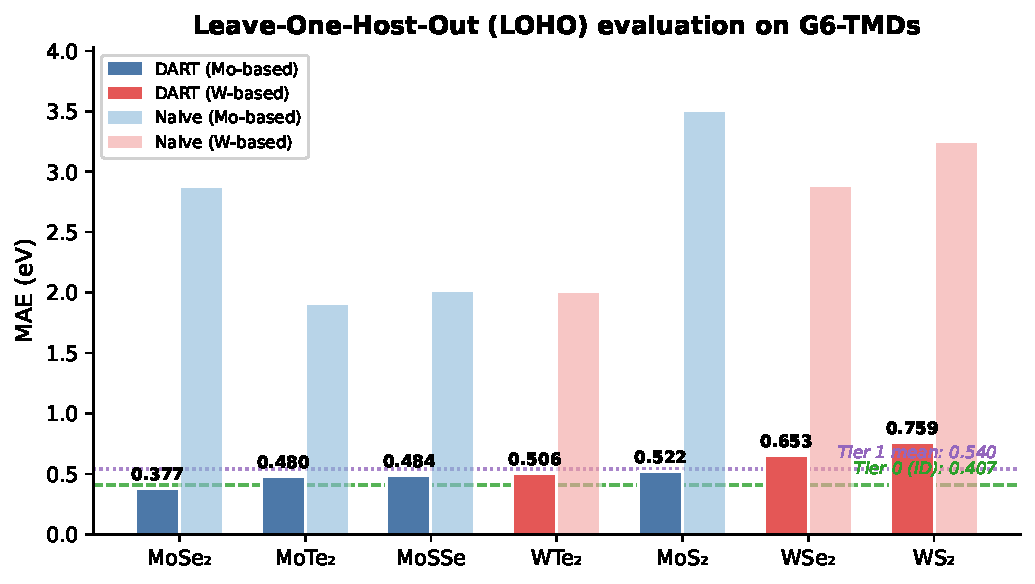
\includegraphics[width=\columnwidth]{figures/loho_bar.pdf}
\caption{Leave-one-host-out (LOHO) evaluation on G6-TMDs.
  Blue bars: Mo-based hosts; red bars: W-based hosts.
  Faded bars: naive (training-set mean) baseline.
  Dashed green line: Tier~0 (in-distribution) MAE;
  dotted purple line: Tier~1 mean.}
\label{fig:loho}
\end{figure}

%----------------------------------------------------------------------
\subsection{Compositional OOD evaluation (Tier~2)}\label{sec:blockout}
%----------------------------------------------------------------------

The G6$\times$3d block-out experiment holds out all (G6-host, 3d-dopant)
pairs, testing whether \dart{} can perform matrix completion for unseen
host--dopant combinations.
The overall MAE is 0.534\eV{}, comparable to Tier~1 (0.540\eV{}),
demonstrating that \dart{}'s compositional generalization matches its
host-transfer capability.

%----------------------------------------------------------------------
\subsection{ct-UAE transfer embedding analysis}\label{sec:uae}
%----------------------------------------------------------------------

We ablate the ct-UAE pretrained atomic embeddings under OOD conditions
(Table~\ref{tab:uae}).

\begin{table}[t]
\centering
\caption{ct-UAE ablation under Tier~1 LOHO.
  $p$-values from paired $t$-test and Wilcoxon signed-rank test
  over 7 folds.}
\label{tab:uae}
\begin{tabular}{@{}lcc@{}}
\toprule
 & with ct-UAE & without ct-UAE \\
\midrule
Tier~0 (ID) MAE        & \textbf{0.407} & 0.412 \\
Tier~1 (OOD) mean MAE  & 0.540          & \textbf{0.493} \\
\midrule
Paired $t$-test $p$    & \multicolumn{2}{c}{0.22} \\
Wilcoxon $p$           & \multicolumn{2}{c}{0.38} \\
\bottomrule
\end{tabular}
\end{table}

While ct-UAE provides a modest benefit in-distribution ($-0.005$\eV{}),
the trend reverses under OOD: removing ct-UAE \emph{improves} the mean
LOHO MAE by 0.047\eV{}, though neither difference reaches statistical
significance.
We hypothesize that ct-UAE embeddings, pretrained on bulk crystals from
the Materials Project, encode chemical priors that are partially
misaligned with the 2D defect domain---a cautionary finding for
transfer-learning practitioners.

%----------------------------------------------------------------------
\subsection{Uncertainty quantification}\label{sec:uq}
%----------------------------------------------------------------------

The 7-model ensemble provides calibrated uncertainty estimates after
temperature scaling ($\tau = 2.57$).
At the 90\% nominal coverage level, the empirical coverage reaches
93.4\%, with an expected calibration error (ECE) of 0.068.
The Spearman correlation between predicted uncertainty ($\sigma$) and
absolute error is 0.577 ($p < 10^{-5}$), confirming that ensemble
variance is a meaningful, if imperfect, proxy for prediction confidence
(Fig.~\ref{fig:uq}).

\begin{figure*}[t]
\centering
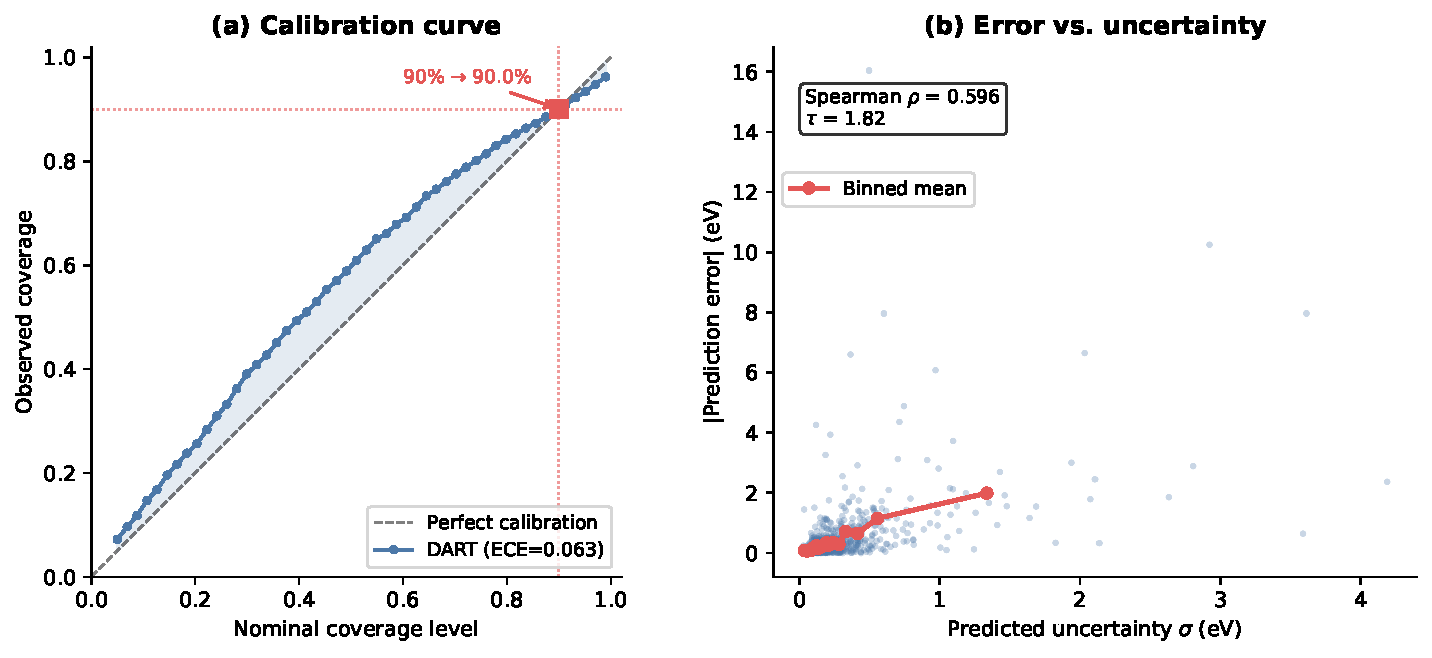
\includegraphics[width=0.85\textwidth]{figures/uq_calibration.pdf}
\caption{Uncertainty quantification performance.
  (a)~Calibration curve: observed vs.\ nominal coverage after temperature
  scaling; the red square marks the 90\% target.
  (b)~Absolute error vs.\ predicted $\sigma$; red points show binned means,
  confirming that higher $\sigma$ correlates with larger errors
  (Spearman $\rho = 0.58$).}
\label{fig:uq}
\end{figure*}

%----------------------------------------------------------------------
\subsection{Physical interpretability}\label{sec:interpret}
%----------------------------------------------------------------------

\paragraph{Defect hub effect.}
Extracting attention weights from the global layers reveals that the
defect atom consistently receives ${\sim}32\times$ higher attention than
host atoms.
This emergent behavior---not explicitly programmed---mirrors the physical
reality that the dopant is the primary source of structural and electronic
perturbation.

\paragraph{Occlusion attribution.}
Masking the defect atom and re-evaluating the model yields a mean absolute
prediction shift of 90.7\% of the original $\ef$, confirming that the
model's predictions are overwhelmingly driven by defect-site information.
